\subsubsection*{2.a}
On affiche la structure des tables ALL\_TAB\_COLUMNS, USER\_USERS,
ALL\_CONSTRAINTS et USER\_TAB\_PRIVS avec desc

\lstinputlisting[style=sqlstyle]{SQL/Partie5/desc.sql}

\begin{center}
    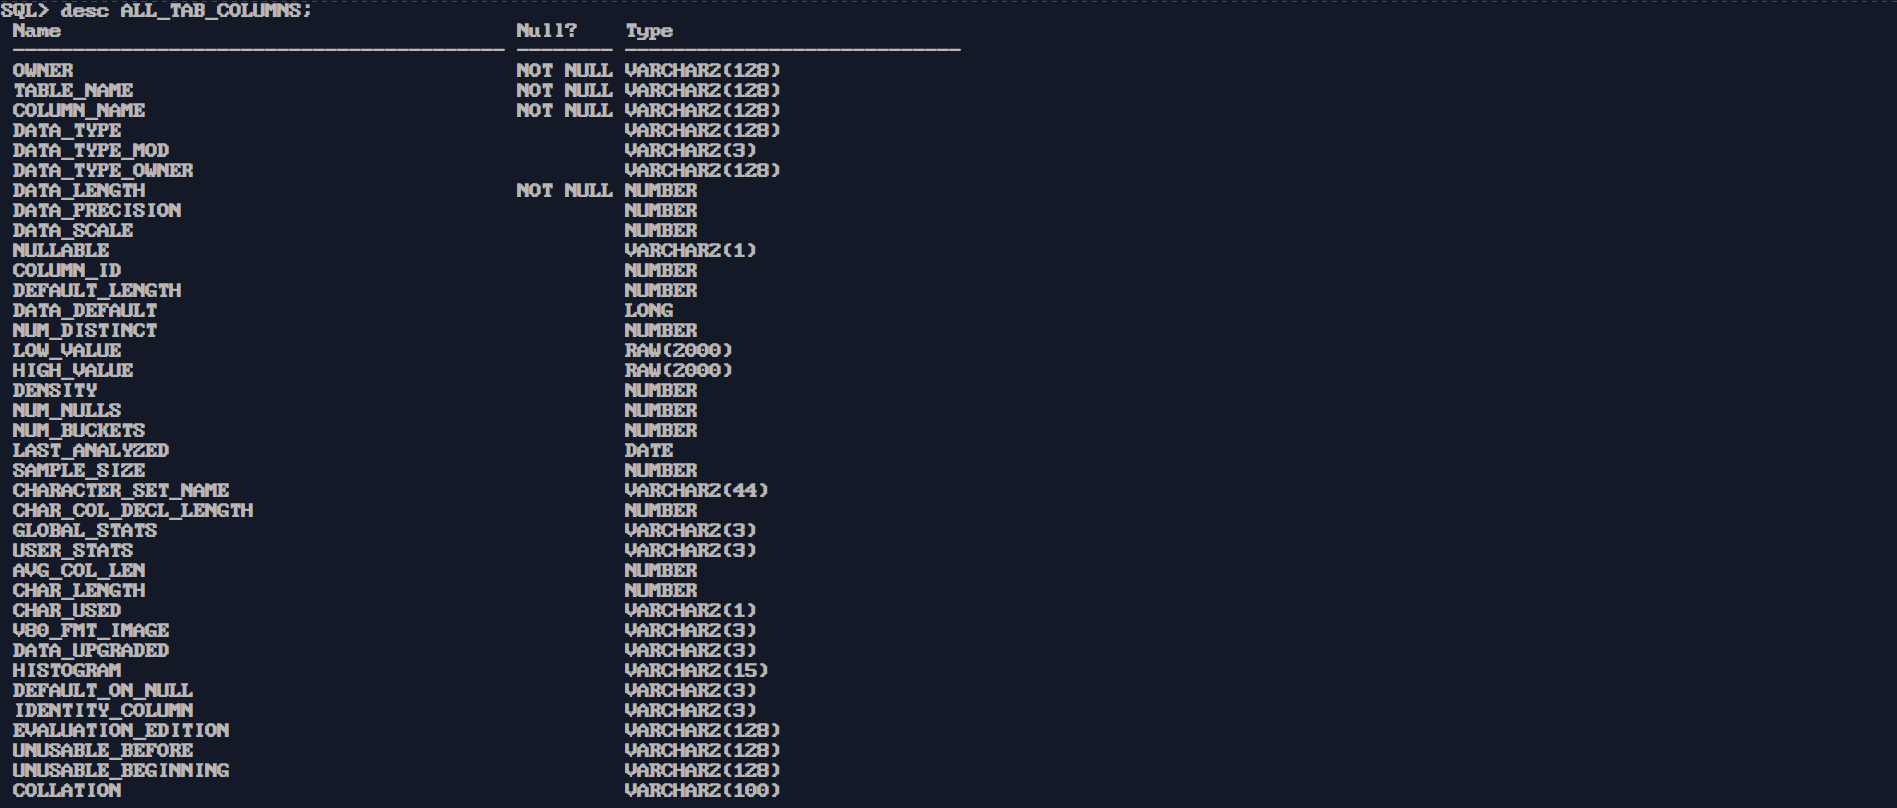
\includegraphics[width=\textwidth]{ScreenShot/Partie5/desc1.png}
\end{center}

\begin{center}
    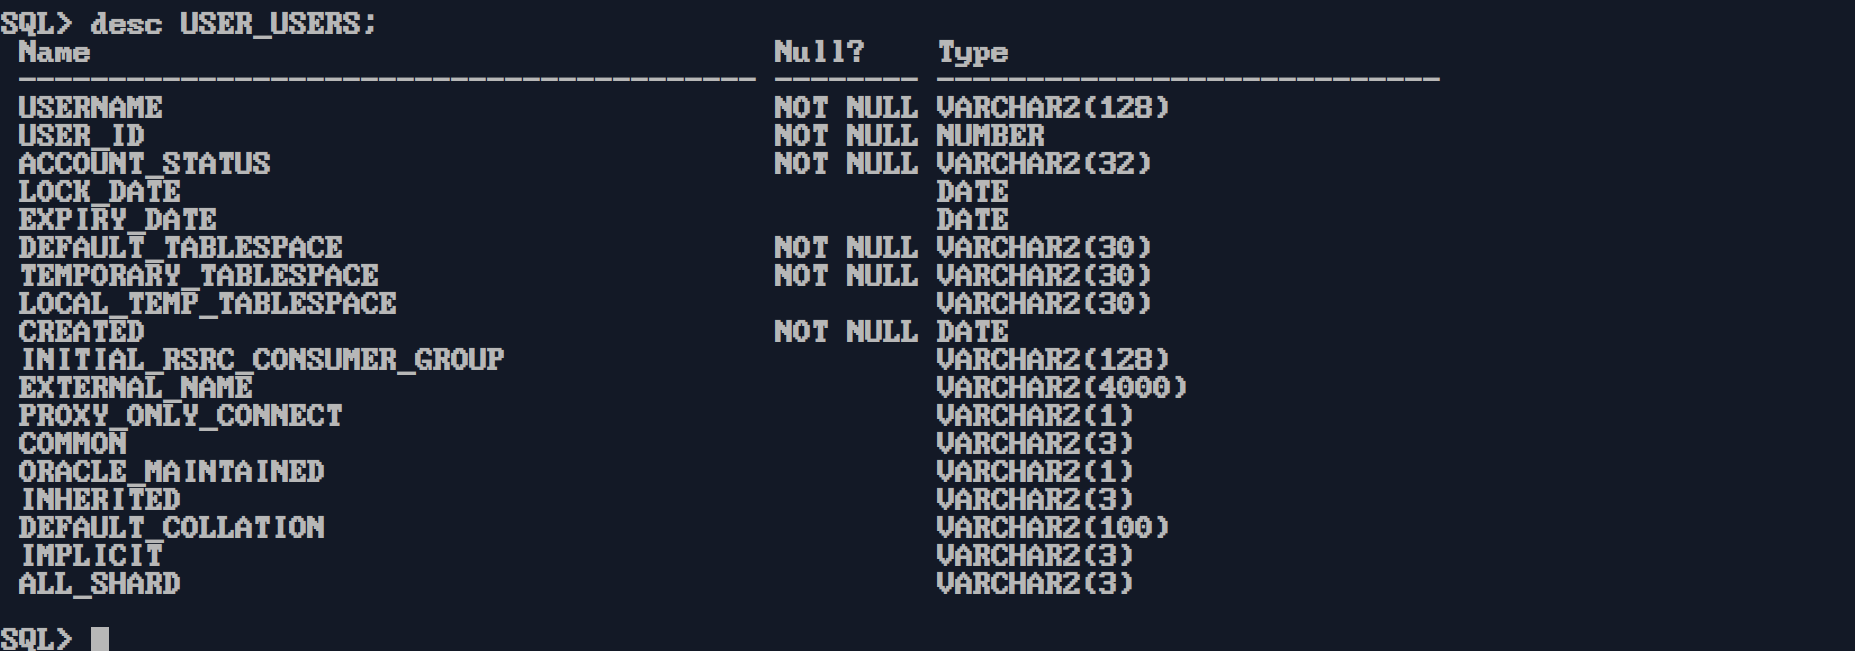
\includegraphics[width=\textwidth]{ScreenShot/Partie5/desc2.png}
\end{center}


\begin{center}
    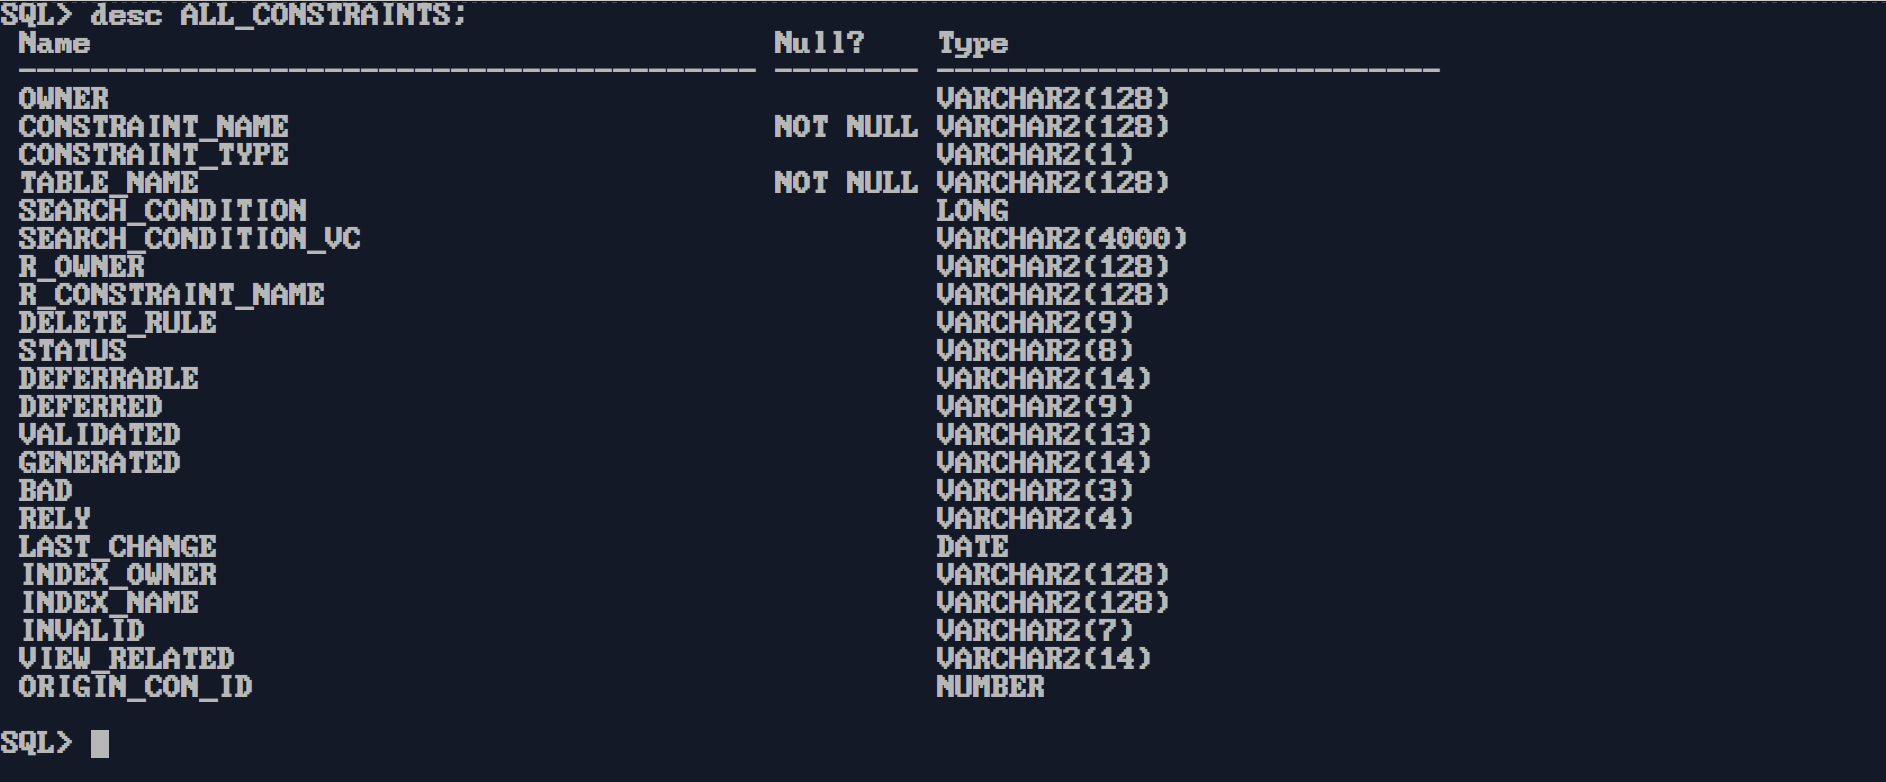
\includegraphics[width=\textwidth]{ScreenShot/Partie5/desc3.png}
\end{center}


\begin{center}
    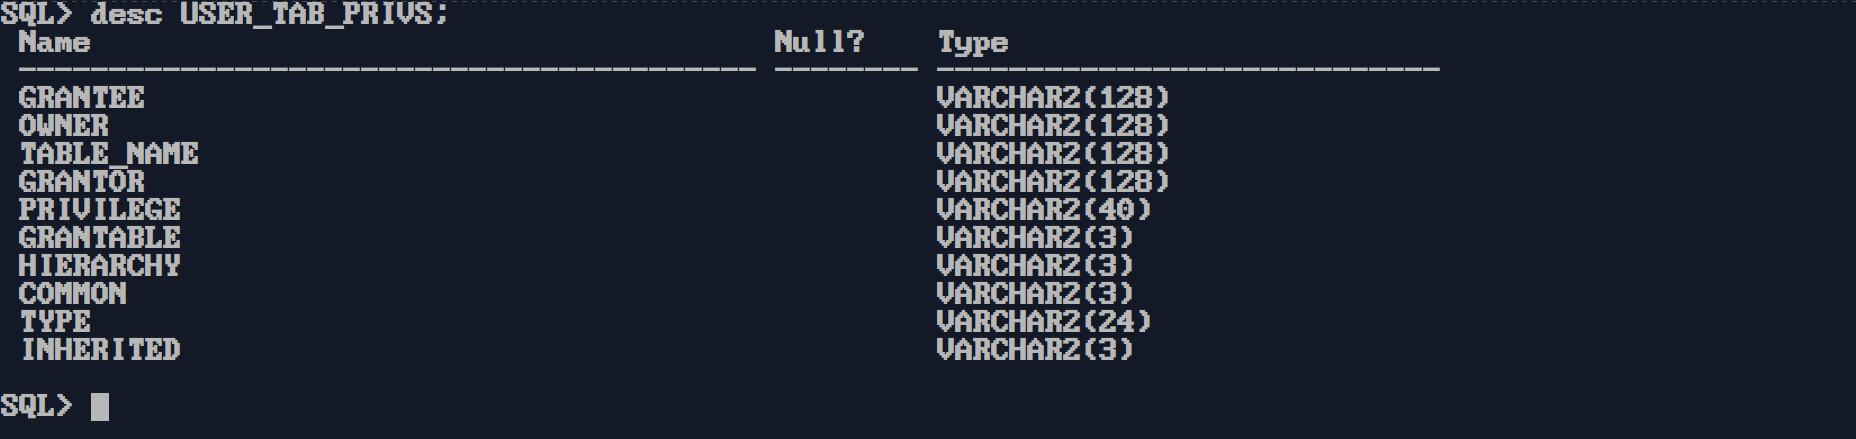
\includegraphics[width=\textwidth]{ScreenShot/Partie5/desc4.png}
\end{center}


\subsubsection*{2.b}

\begin{prettyBox}{Role}{myblue}
\begin{itemize}
    \item \textbf{ALL\_TAB\_COLUMNS} : stocke les colonnes de toutes les vues et tables accessibles à chaque utilisateur.
    \item \textbf{USER\_USERS} : contient une description de l'utilisateur actuellement connecté.
    \item \textbf{ALL\_CONSTRAINTS} : contient toutes les contraintes accessibles à chaque utilisateur.
    \item \textbf{USER\_TAB\_PRIVS} : contient les privilèges objets des tables de l'utilisateur actuellement connecté.
\end{itemize}
\end{prettyBox}

